% Farbkarte TU Darmstadt: http://www.webteam.tu-darmstadt.de/media/webteam_wissensdatenbank/artikel_1/farbkarte_TU_Darmstadt.png
\documentclass[nochapterpage,nopartpage,noheadingspace,numbersubsubsec,bigchapter,colorback,accentcolor=tud9c,10pt]{tudreport}
\usepackage[ngerman,english]{babel}

\usepackage[stable]{footmisc}
\usepackage[ngerman,english]{hyperref}

\usepackage{longtable}
\usepackage{multirow}
\usepackage{booktabs}

% Custom packages
\usepackage{wrapfig}
\usepackage{etoolbox}
\usepackage{multicol}
\usepackage{listings}

\lstset{
    breaklines=true,
    postbreak=\raisebox{0ex}[0ex][0ex]{\ensuremath{\color{red}\hookrightarrow\space}}
}

% Reset chapter counter after introducing a new part and start chapters on the same page
\makeatletter
\@addtoreset{chapter}{part}
\patchcmd{\scr@startchapter}{\if@openright\cleardoublepage\else\clearpage\fi}{}{}{}
\makeatother

\hypersetup{%
  pdftitle={Internet Praktikum TK Documentation},
  pdfauthor={M. Schanz},
  pdfsubject={Project Documentation},
  pdfview=FitH,
  pdfstartview=FitV
}

%%% Zum Tester der Marginalien %%%
  \newif\ifTUDmargin\TUDmarginfalse
  %%% Wird der Folgende Zeile einkommentiert,
  %%% werden Marginalien gesetzt.
  % \TUDmargintrue
  \ifTUDmargin\makeatletter
    \TUD@setmarginpar{2}
  \makeatother\fi
%%% ENDE: Zum Tester der Marginalien %%%

\newlength{\longtablewidth}
\setlength{\longtablewidth}{0.7\linewidth}
\addtolength{\longtablewidth}{-\marginparsep}
\addtolength{\longtablewidth}{-\marginparwidth}

\title{Internet Praktikum TK 2016\\ Conference Management System\\ Team Whisky}
\subtitle{Auel, Tarek,\\ Sahin, Huzeyfe\\ Schanz, Markus}


\begin{document}
\maketitle
\tableofcontents
%\listoffigures
%\addcontentsline{toc}{chapter}{\listfigurename}


\part{User Documentation}
\label{part:user}

  \chapter{Introduction}
  \label{ch:user:intro}

A conference management system is a web application for organizing and managing conferences. In such a system, users are allowed to upload submissions, review these submissions with a feedback or change the conference information itself. This implies that users have different roles during a conference such as attendee, author, reviewer and chair to be able to perform their tasks. The user documentation shows how to perform the aforementioned tasks.

  \chapter{User}

User is the initial role after the registration without any joined conferences.

	\section{Create an account}

%Creating an account allows the user to be part of the conference management system. Follow the steps below to create an account.

\begin{enumerate}
	\item	Click on the \textbf{Create new account} link on the main page. (see figure \ref{fig:main-page})
	\item	Enter the first name, last name, email, username, affiliation, password and confirm password.
	\item	Click on the \textbf{Submit} button to process the registration.
\end{enumerate}

%\begin{enumerate}
%	\item	Click on the \textbf{Create new account} link on the main page. (see figure \ref{fig:main-page})
%	\item	Fill out the form respectively to their labels.
%	\item	Click on the \textbf{Submit} button.
%\end{enumerate}

	\section{Manage profile}

%Editing a profile allows the user to change the personal information, changing the password and deleting the account. Follow the steps below to edit the profile.

\begin{enumerate}
	\item	Log in to your account. Navigate to the drop-down box located in the top right corner and open it by clicking on \textbf{your name}. Locate \textbf{Manage Profile} and click on it. (see figure \ref{fig:user-menu}, box \#1)
	\item	Once on \textbf{Manage Profile}, change your first name, last name, email, username, street, postal code, city, state, country or affiliation.
	\item	Click on the \textbf{Edit Profile} button to save the changes.
\end{enumerate}

%\begin{enumerate}
%	\item	Log in to your account. Navigate to \textbf{your name}, then click on {Manage Profile}. (see figure \ref{fig:user-menu})
%	\item	Once on \textbf{Manage Profile}, change the desired input from the form respectively to their labels.
%	\item	Click on the \textbf{Edit Profile} button.
%\end{enumerate}


  \chapter{Attendee}

Attendees are users who are part a conference after registering into the conference management system and joining a conference.

	\section{Join conference}

%Joining a conference allows the user to be part of a public or private conference as an attendee at time. Follow the steps below to join a conference

\begin{enumerate}
	\item	Log in to your account. Navigate to the drop-down box located in the top right corner and open it by clicking on \textbf{your name}. Locate  \textbf{Join Conference} and click on it. (see figure \ref{fig:user-menu}, box \#3)
	\item	Select a conference from the drop-down list and enter the shared secret key.
	\item	Click on the \textbf{Join Conference} button to join the selected conference.
\end{enumerate}

  \chapter{Author}

Authors are allowed to create submissions for a conference in order to submit their papers during the submission phase.

	\section{Create submission}

%Creating a submission is a functionality targeted for authors only. Authors are only allowed to submit their papers for a conference during the submission phase. Follow the steps below to create a submission.

\begin{enumerate}
	\item	Log in to your account. Navigate to the drop-down box located in the top and open it by clicking on \textbf{Submissions}. Locate \textbf{Create Submission} and click on it. (see figure \ref{fig:submission-menu})
	\item	Enter the title, abstract and keywords of the submission.
	\item	Select multiple authors from the drop-down list if necessary.
	\item	Either drag and drop your paper into the drop zone or click on the drop zone to select the file from your local machine. \textbf{*}
	\item	Click on the \textbf{Submit Paper} button to create the submission.
\end{enumerate}

%\begin{enumerate}
%	\item	Log in to your account. Navigate to \textbf{Submissions}, then click on \textbf{Create Submission}.  (see figure \ref{fig:submission-menu})
%	\item	Fill out the form respectively to their labels.
%	\item	Click on the \textbf{Submit Paper} button.
%\end{enumerate}

\textbf{*Please note:} PDF format only.


  \chapter{Reviewer}

Reviewer are allowed to create reviews for their assigned submissions and give feedback during the review phase, which is assignable by the chair only.

	\section{Create review}

%Creating a review is a functionality targeted for reviewer only. Reviewer are allowed to review assigned submissions for a conference during the review phase. Follow the steps below to create a review.

\begin{enumerate}
	\item	Log in to your account. Navigate to the drop-down box located in the top and open it by clicking on \textbf{Reviews}. Locate \textbf{Overview} and click on it. (see figure \ref{fig:review-menu})
	\item	Once in \textbf{Overview}, click on the {Review} button from a submission. (see figure \ref{fig:review-overview})
	\item	Select only one option for both your expertise and overall evaluation.
	\item	Enter the evaluation summary, major strong points, major weak points, detailed comments.
	\item	Select between the draft or finished option.
	\item	Click on the \textbf{Submit Review} button to create the review.
\end{enumerate}

%\begin{enumerate}
%	\item	Log in to your account. Navigate to \textbf{Reviews}, then click on \textbf{Overview}.  (see figure \ref{fig:review-menu})
%	\item	Once in \textbf{Overview}, click on the {Review} button from a submission.  (see figure \ref{fig:review-overview})
%	\item	Fill out the form respectively to their labels.
%	\item	Click on the \textbf{Submit Review} button.
%\end{enumerate}

  \chapter{Chair}

Chairs are allowed to manage the conference, users and submissions. Chairs can edit conference information such as submission deadlines, review deadlines or general information. He can also assign roles to specific users or assign reviewer to submissions, who are part of his conference. 

	\section{Manage conference}

%Managing conferences is also a task assigned to the chair only. The chair is able to change his conference information such as the name, submission- or review deadlines. Follow the steps below to manage a conference.

\begin{enumerate}
	\item	Log in to your account. Navigate to the drop-down box located in the top right corner and open it by clicking on \textbf{your name}. Locate \textbf{My Conferences} and click on it. (see figure \ref{fig:user-menu}, box \#2)
	\item	Once in \textbf{My Conferences}, click on the Manage Conference link one of your conferences. (see figure \ref{fig:conference-overview})
	\item	To change the conference information, enter the conference name, shared secret and conference description.
	\item	Click on the calendar symbol next to the submission and/or review deadline to select a date from the calendar. *
	\item	Click on the \textbf{Save Conference} button to save the conference changes.
\end{enumerate}

	\section{Manage user roles}

%Managing users from a conference is a task assigned to the chair only. The chair is able to assign roles to registered users who are part of his conference. Follow the steps below to manage users.

\begin{enumerate}
	\item	Log in to your account. Navigate to the drop-down box located in the top and open it by clicking on \textbf{Conference Management}. Locate \textbf{Users} and click on it. (see figure \ref{fig:conference-menu}, box \#2)
	\item	Enter the name of an attendee as a filter and/or select the role of the user if necessary.
	\item	Click on the switch to assign or revoke role/s to a user.
\end{enumerate}

%\begin{enumerate}
%	\item	Log in to your account. Navigate to \textbf{your name}, then click on \textbf{My Conferences}. (see figure \ref{fig:user-menu-chair})
%	\item	Once in \textbf{My Conferences}, click on the Manage Conference link one of your conferences. (see figure \ref{fig:conference-overview})
%	\item	Make the desired change from the form respectively to their labels.
%	\item	Click on the \textbf{Save Conference} button.
%\end{enumerate}

\textbf{*Please note:} submission deadline is not allowed to be later than review deadline.

	\section{Assign reviewer to submissions}

\begin{enumerate}
	\item	Log in to your account. Navigate to the drop-down box located in the top and open it by clicking on \textbf{Conference Management}. Locate \textbf{Assign Reviewer} and click on it. (see figure \ref{fig:conference-menu}, box \#1)
	\item	Enter the name of an available reviewer from the drop-down list or select directly one from the drop-down list.
	\item	Click on the \textbf{Save Changes} button to assign the reviewer/s to the submission.
\end{enumerate}


\part{Appendix}
\label{part:appendix}

  \chapter*{A.\quad Application Installation}
  \addcontentsline{toc}{chapter}{A.\quad Application Installation}
  \label{ch:appendix:setup}

    The application does not enforce the usage of a specific operating system. However, we recommend to use a Linux system with a package manager in order to install the required prerequisites to make the setup process as smooth as possible.

  \section*{Prerequisites}
  \label{sec:appendix:setup:prerequisites}

    Before starting with the installation process, please make sure that your system does met the following prerequisites:
        \begin{multicols}{2}
        \begin{itemize}
            \item Git $\ge$ 2.x
            \item Node.js $\ge$ 4.2.x
            \item npm $\ge$ 3.x (part of Node.js)
        \end{itemize}
        \end{multicols}

    \noindent The project heavily relies on strongloop for generating API code as well as on bower to fetch 3rd party java-script libraries. To install both on your system execute the following command:
        \begin{lstlisting}[language=bash]
    # npm install -g strongloop bower
        \end{lstlisting}

  \section*{Installation}
  \label{sec:appendix:setup:install}

    \noindent Use the git command to fetch a copy of the source code repository.%
    \footnote{Requires read access to the repository.}
    The command should be executed by the user who is supposed to run the application and inside an empty directory which is going to hold the application source code.
        \begin{lstlisting}[language=bash]
    $ git clone ssh://git@scm.informatik.tu-darmstadt.de/iptk-ss2016/iptk-ss2016-team-whiskey.git .
        \end{lstlisting}
    For further installation instructions, please stick to the \emph{readme.md} file which is now found inside the directory.


  \chapter*{B.\quad Database Entity Relationship Model}
  \addcontentsline{toc}{chapter}{B.\quad Database Entity Relationship Model}

    % Figure of ERM goes here

  \chapter*{C.\quad Application Screenshots}
  \addcontentsline{toc}{chapter}{C.\quad Application Screenshots}

    % Figure of ERM goes here

        \begin{figure}
            \centering
            \fbox{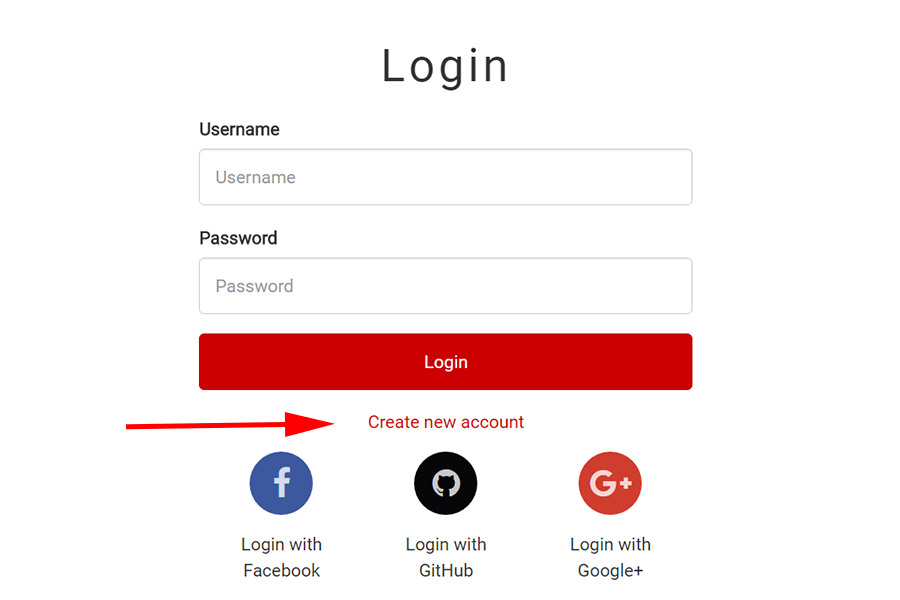
\includegraphics[width=0.9\textwidth]{screenshots/1-main.png}}
            \caption{Main page}
            \label{fig:main-page}
        \end{figure}

        \begin{figure}
            \centering
            \fbox{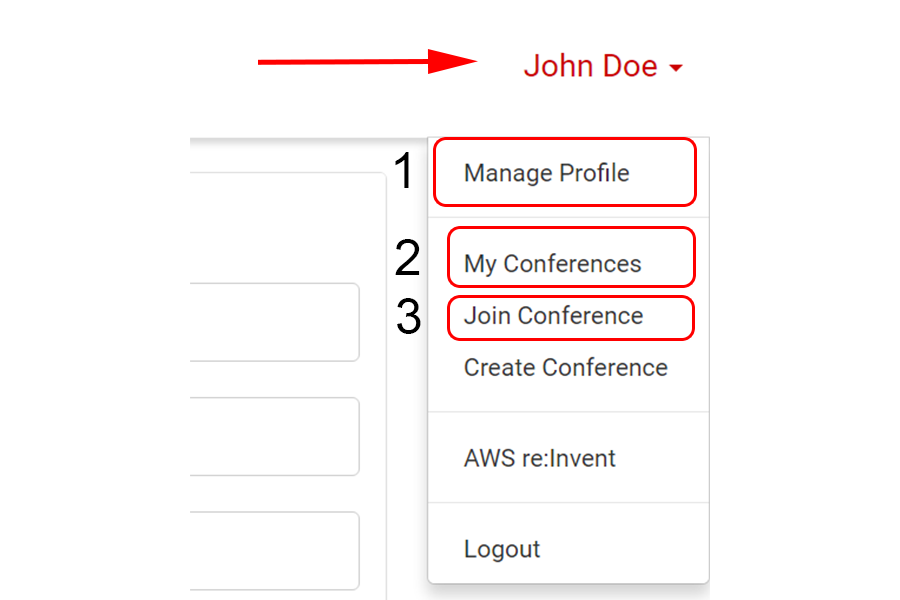
\includegraphics[width=0.9\textwidth]{screenshots/2-user-menu.png}}
            \caption{User menu}
            \label{fig:user-menu}
        \end{figure}

        \begin{figure}
            \centering
            \fbox{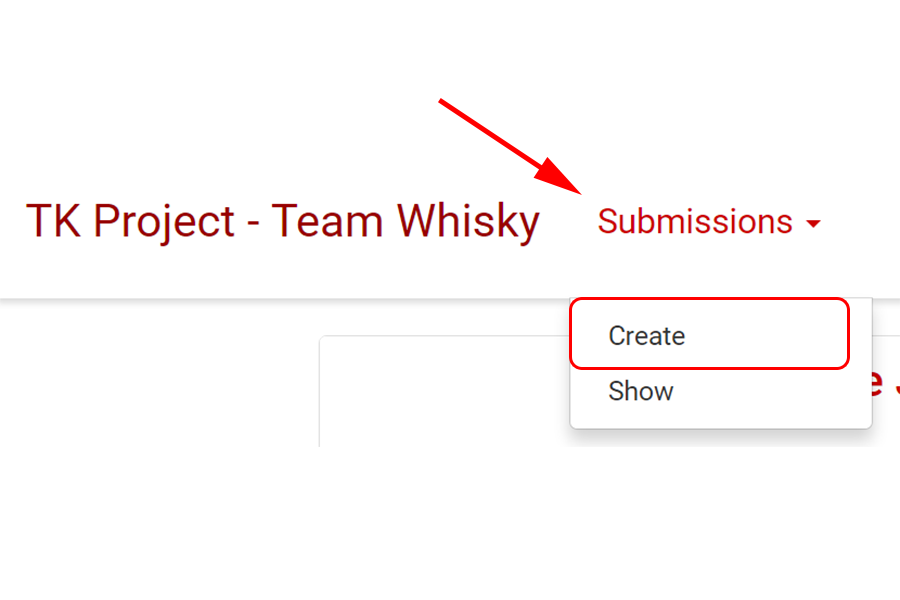
\includegraphics[width=0.9\textwidth]{screenshots/3-submission-menu.png}}
            \caption{Submission menu}
            \label{fig:submission-menu}
        \end{figure}

        \begin{figure}
            \centering
            \fbox{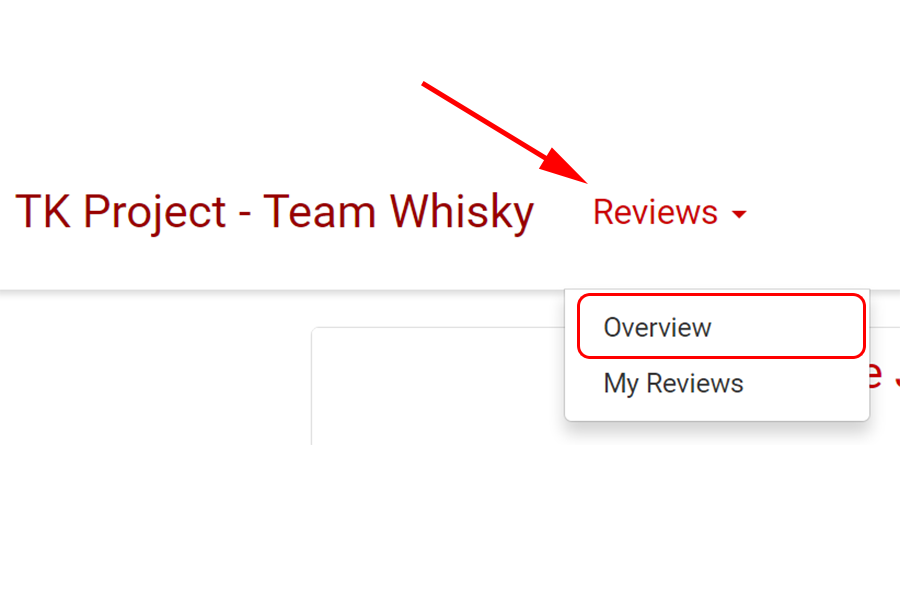
\includegraphics[width=0.9\textwidth]{screenshots/4-review-menu.png}}
            \caption{Review menu}
            \label{fig:review-menu}
        \end{figure}

        \begin{figure}
            \centering
            \fbox{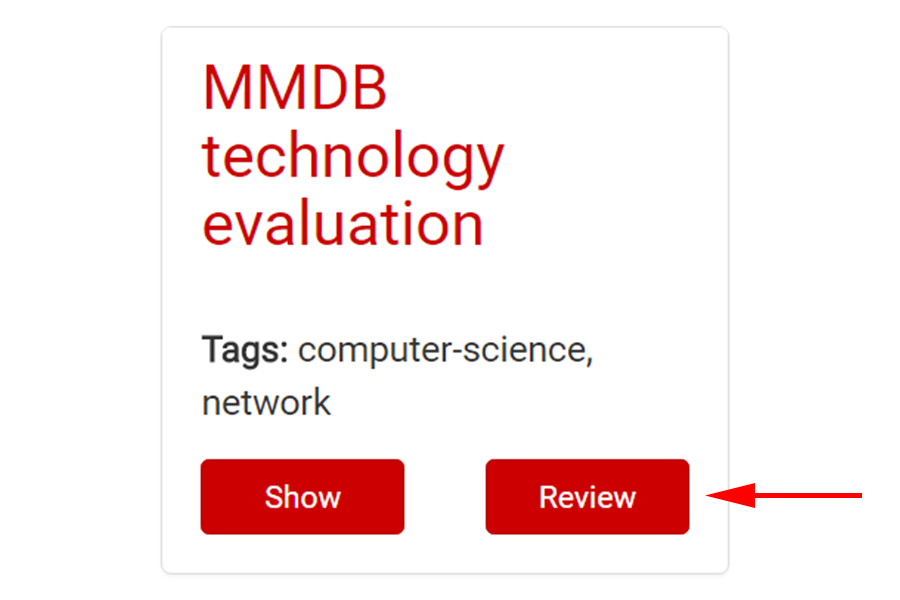
\includegraphics[width=0.9\textwidth]{screenshots/5-review-overview.png}}
            \caption{Review overview}
            \label{fig:review-overview}
        \end{figure}

        \begin{figure}
            \centering
            \fbox{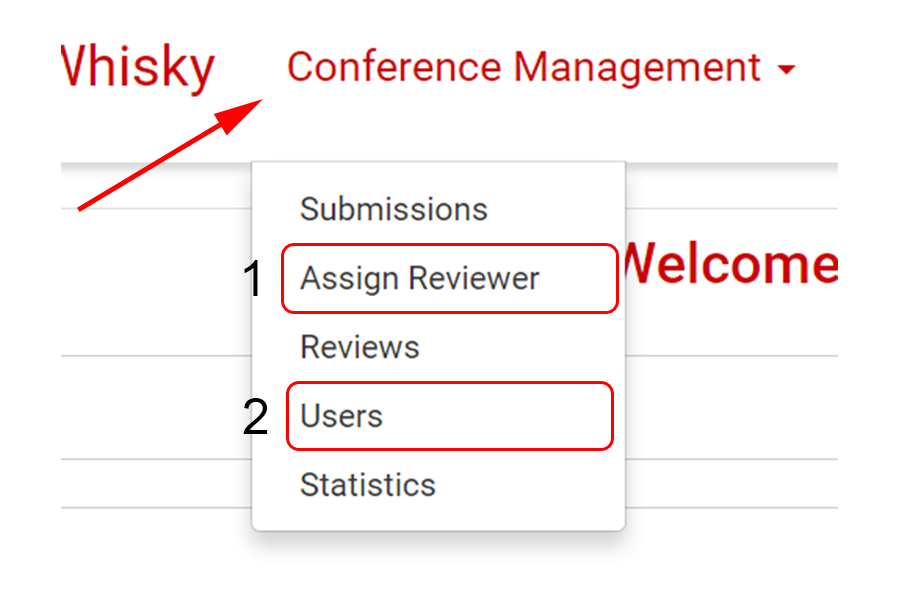
\includegraphics[width=0.9\textwidth]{screenshots/6-conference-menu.png}}
            \caption{Conference menu}
            \label{fig:conference-menu}
        \end{figure}

        \begin{figure}
            \centering
            \fbox{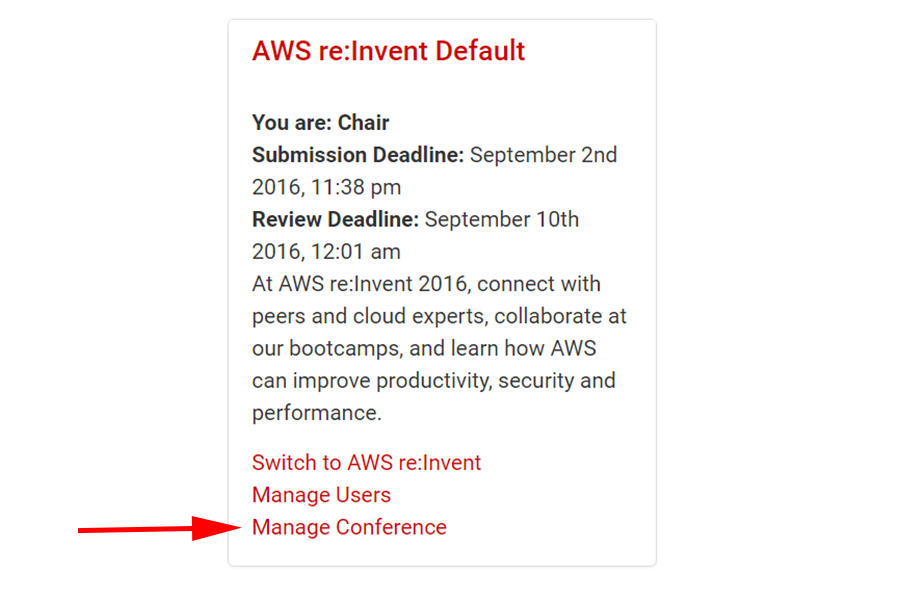
\includegraphics[width=0.9\textwidth]{screenshots/7-conference-overview.png}}
            \caption{Conference overview}
            \label{fig:conference-overview}
        \end{figure}

  \chapter*{D.\quad (Un)Implemented Features}
  \addcontentsline{toc}{chapter}{D.\quad (Un)Implemented Features}

    % List of features goes here
    Below is the list of (un)implemented features, copied from the SCM wiki page.%
    \footnote{\url{https://scm.informatik.tu-darmstadt.de/projects/iptk-ss2016/wiki/Conference_management_system_-_Features}}
    A checked box ($\boxtimes$) means that the feature is implemented whereas an unchecked box ($\square$) means that the feature is (partly) unimplemented
        \begin{itemize}
            \setlength\itemsep{0em}
            \item Roles
            \begin{itemize}
                \item[$\boxtimes$] Authors [0..*]
                \item[$\boxtimes$] Reviewers [0..*]
                \item[$\boxtimes$] Chair [1..*]
            \end{itemize}

            \item General
            \begin{itemize}
                \item[$\boxtimes$] responsive design: access the web application with different kinds of devices (mobile, tablet, pc..)
            \end{itemize}

            \item As a user, I can
            \begin{itemize}
                \item[$\boxtimes$] register to the system at least with email, password
                \begin{itemize}
                    \item[$\boxtimes$] emails are unique
                    \item[$\boxtimes$] users can have multiple roles (e.g., author and reviewer)
                    \item[$\boxtimes$] additional information (see slides)
                    \begin{itemize}
                        \item[$\boxtimes$] e.g., basic profile (given name, family name, postal address)
                        \item[$\boxtimes$] e.g., affiliation (institution, city, state, country)
                    \end{itemize}
                \end{itemize}
                \item[$\boxtimes$] login to the system at least with registered email, password
                \item[$\boxtimes$] edit my profile (password, additional information)
                \item[$\boxtimes$] remove my profile
                \item[$\boxtimes$] logout
            \end{itemize}

            \item As a author, I can
            \begin{itemize}
                \item[$\boxtimes$] create a new submission (if submission is open)
                \begin{itemize}
                    \item[$\boxtimes$] title
                    \item[$\boxtimes$] registered authors [1..*] (given name, family name, email affiliation)
                    \item[$\boxtimes$] abstract
                    \item[$\boxtimes$] keywords (multi-selection) that describe the submission (e.g., research fields)
                    \item[$\boxtimes$] upload the paper (.pdf)
                \end{itemize}
                \item[$\boxtimes$] access current submissions (overview)
                \begin{itemize}
                    \item[$\square$] status: incompleted, completed, closed, accepted, rejected
                \end{itemize}
                \item[$\boxtimes$] look at a submission
                \item[$\boxtimes$] edit a submission (if submission is open)
                \item[$\boxtimes$] withdraw a submission
            \end{itemize}

            \item As a reviewer, I can
            \begin{itemize}
                \item[$\boxtimes$] access assigned submissions (overview + status)
                \item[$\boxtimes$] look at an assigned submission
                \begin{itemize}
                    \item[$\boxtimes$] details, pdf download or view
                \end{itemize}
                \item[$\boxtimes$] make a review > template (if review is open)
                \begin{itemize}
                    \item[$\boxtimes$] reviewer expertise: (1) not familar w/ the topic - (5) expert
                    \item[$\boxtimes$] overall evaluation: (1) strong reject - (5) strong accept
                    \item[$\boxtimes$] summary
                    \item[$\boxtimes$] major strong popints
                    \item[$\boxtimes$] major weak points
                    \item[$\boxtimes$] detailed comments
                \end{itemize}
                \item[$\boxtimes$] edit a review (if reviewing phase is open)
            \end{itemize}

            \item As a chair, I can
            \begin{itemize}
                \item[$\boxtimes$] list all paper submissions
                \begin{itemize}
                    \item[$\boxtimes$] look at a submissions (details, pdf download or view)
                    \item[$\square$] withdraw a submission
                \end{itemize}
                \item[$\boxtimes$] list all authors
                \begin{itemize}
                    \item[$\boxtimes$] look at detail information
                \end{itemize}
                \item[$\boxtimes$] list all reviewers
                \begin{itemize}
                    \item[$\boxtimes$] look at detail information
                \end{itemize}
                \item[$\boxtimes$] list all reviews
                \begin{itemize}
                    \item[$\boxtimes$] look at a review
                \end{itemize}
                \item[$\boxtimes$] assign papers to reviewers
                \begin{itemize}
                    \item[$\boxtimes$] conflict avoidance: an author is not allow to review his own paper
                \end{itemize}
                \item[$\boxtimes$] do the schedule management
                \begin{itemize}
                    \item[$\boxtimes$] automatic: set close deadlines for submissions and reviews
                    \item[$\boxtimes$] manual: (re-)open/close submissions and reviews
                \end{itemize}
                \item[$\square$] view fancy summary charts or reports (e.g., total submission, acceptances, topics, countries etc.)
            \end{itemize}

            \item Bonus features (OPTIONAL)
            \begin{itemize}
                \item[$\square$] users must confirm their registration by clicking on a registration link sent via email
                \item[$\square$] email notification to submitters and reviewers (status changes)
                \item[$\square$] chat with other online authors
                \item[$\square$] automatic assignment (even distribution) and conflict resolving
                \item[$\boxtimes$] a user can create multiple conference events and becomes the chair (=administrator) of them
            \end{itemize}
        \end{itemize}

\end{document}
